\documentclass{article}

\usepackage[a4paper, total={7in, 10in}]{geometry}

\usepackage{amsmath}
\usepackage{subcaption}
\usepackage{graphicx}
\graphicspath{{../Results/Protected/}}

\title{AIMS Course 1: Data, Estimation and Inference}
\author{Jake Levi}
\date{October 2022}

\begin{document}
\maketitle

% Section: introduction

\section{Introduction}

This lab report investigates the use of Gaussian Processes, a type of machine learning model motivated by Bayesian probability theory, for modelling a meteorological dataset called Sotonmet. In a Gaussian Process model, given a mean function $\mu$, kernel function $K$, training input data $x$ (represented as a vector), and prediction inputs $x^*$, the noisy training labels $y$ (which we assume are noisy observations of unknown noiseless training labels $f$) and noiseless prediction labels $f^*$ have a joint Gaussian distribution:

% Equation: joint distribution

\begin{equation}
    p\left( \begin{bmatrix}
        y \\
        f^*
    \end{bmatrix} \right)
    = \mathcal{N} \left( \begin{bmatrix}
        y \\
        f^*
    \end{bmatrix} \middle| \begin{bmatrix}
        \mu(x) \\
        \mu(x^*)
    \end{bmatrix}, \begin{bmatrix}
        K(x, x) + \sigma^2 I & K(x, x^*) \\
        K(x, x^*)^T & K(x^*, x^*) \\
    \end{bmatrix} \right)
\end{equation}

Where $K(x, x^*)$ is a matrix whose $(i, j)$th element is given by $K(x, x^*)_{i,j} = K(x_i, x^*_j)$. The predictive distribution $p(f^* \mid y)$ follows from the formula for the conditional distribution of a jointly Gaussian random variable \cite{bishop2006pattern}:

% Equation: conditional distribution

\begin{align}
    p(f^* \mid y) &= \mathcal{N}\left(f^* \mid \mu^*, \Sigma^* \right) \\
    \text{where} \qquad \mu^* &= \mu(x^*) + K(x^*, x) \left( K(x, x) + \sigma^2 I \right)^{-1} (y - \mu(x)) \\
    \Sigma^* &= K(x^*, x^*) - K(x^*, x) \left( K(x, x) + \sigma^2 I \right) ^{-1} K(x, x^*)
\end{align}

The log marginal likelihood (LML) of the noisy training labels $y$ given training input data $x$ (and also implicitly given any hyperparameters of the model) is given by:

% Equation: log marginal likelihood

\begin{equation}
    \log \left( p(y \mid x) \right) = -\frac{1}{2}\log\left(\det \left(2\pi\left( K(x, x) + \sigma^2 I \right)\right)\right) -\frac{1}{2}(y - \mu(x))^T \left( K(x, x) + \sigma^2 I \right)^{-1} (y - \mu(x))
\end{equation}

This expression implies that maximising the LML encourages $\mu(x)$, $K(x,x)$ and $\sigma$ to fit the data accurately and with calibrated uncertainty. Maximising the LML can also be motivated from a Bayesian perspective, which is discussed further in Appendix \ref{appendix:why_lml}.

The focus in this coursework submission is on predicting the tide height given the time of day, for which the the training and ground truth data is shown in Figure \ref{fig:data}, alongside an independent Gaussian Process prediction in Figure \ref{fig:ind_pres}.

% Section: results

\section{Results}

We start off by considering Gaussian processes with constant mean function and squared exponential kernel, whose mean and kernel functions are related to the hyperparameters $c$, $k$, and $\lambda$ as follows ($\sigma$ is also considered to be a hyperparameter, although it is not explicitly part of the mean or kernel functions):

% Equation: constant mean and squared exponential kernel function

\begin{align}
\mu(x) &= c \\
K_{\mathrm{sqe}}(x, x') &= k \exp\left( -\left( \frac{x - x'}{\lambda} \right)^2 \right)
\end{align}

Within the domain of such Gaussian Processes, we start off by considering two Gaussian processes denoted by sqe\_1 and sqe\_2, as described in Table \ref{table:sqe_table}. Samples from the prior distributions of sqe\_1 and sqe\_1 are shown in Figure \ref{fig:prior_samples}, which show that the prior distribution of sqe\_1 looks subjectively like a much more plausible explanation for the data. The predictive distributions of these Gaussian Processes are shown in Figure \ref{fig:pred_distribution}, which show that, although sqe\_1 produced a \emph{prior} distribution which looks like a more plausible explanation for the training data, sqe\_2 produces a \emph{predictive} distribution which looks like a much better fit to the training data. Furthermore, the predictive distribution of sqe\_1 is "confidently wrong" (the mean is far away from the ground truth labels and with high certainty/low standard deviation) in regions containing ground truth labels but no training data, which could be a very undesirable property to have in a safety-critical prediction scenario. Lastly, samples from the predictive distribution of both Gaussian Processes are shown in Figure \ref{fig:pred_samples}, which show that neither Gaussian Process produces samples that reflect the data distribution particularly well.

\appendix

\section{Figures}\label{appendix:figures}

% Figure: Sotonmet dataset

\begin{figure}[pht]
    \centering
    \subfloat[
        \centering Training and ground truth data
        \label{fig:data}
    ]{
        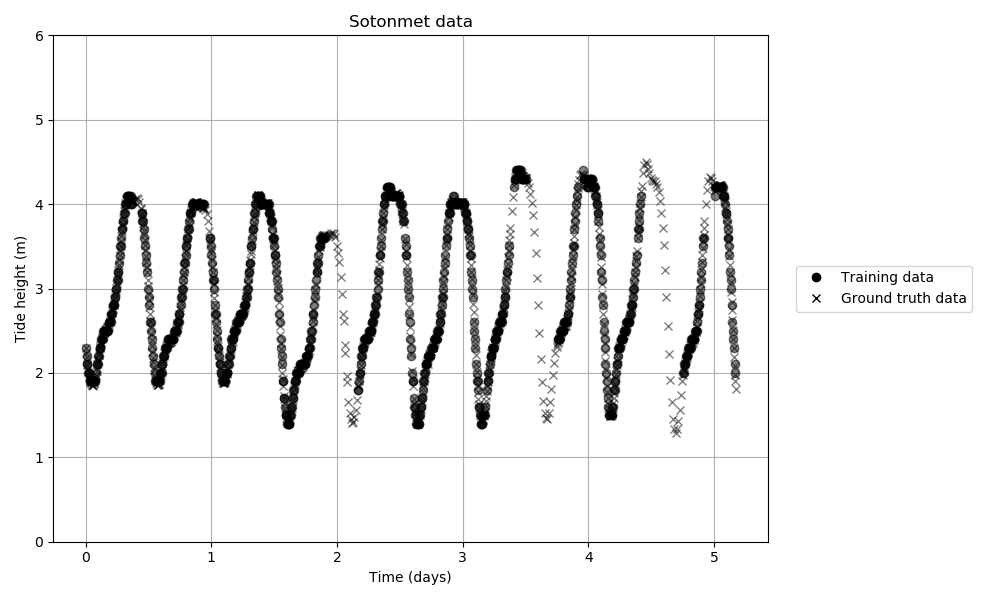
\includegraphics[width=0.45\textwidth]{Sotonmet_data.png}
    }
    \subfloat[
        \centering Independent Gaussian Process predictions
        \label{fig:ind_pres}
    ]{
        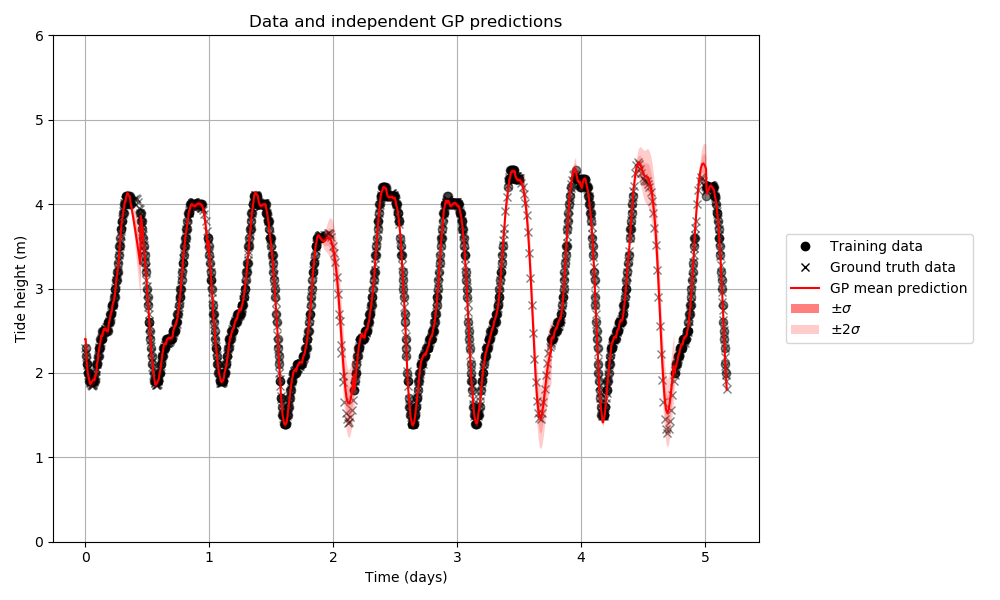
\includegraphics[width=0.45\textwidth]{Data_and_independent_GP_predictions.png}
    }
    \caption{The Sotonmet dataset}
    \label{fig:sotonmet}
\end{figure}

% Figure: samples from SQE prior distribution

\begin{figure}[pht]
    \centering
    \subfloat[
        \centering Samples from the prior of sqe\_1
        \label{fig:prior_sqe_1}
    ]{
        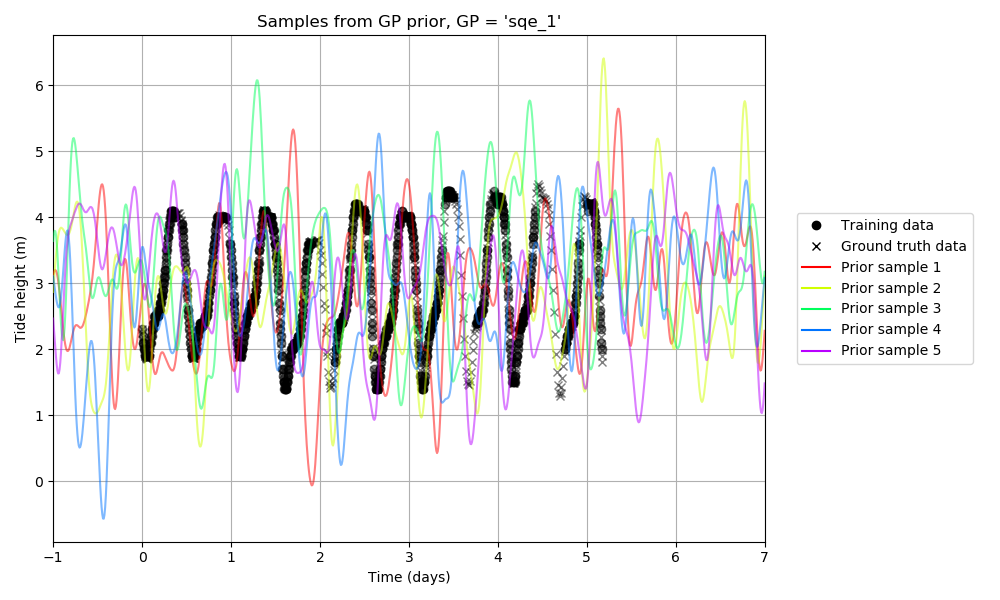
\includegraphics[width=0.45\textwidth]{Samples_from_GP_prior,_GP____sqe_1_.png}
    }
    \subfloat[
        \centering Samples from the prior of sqe\_2
        \label{fig:prior_sqe_2}
    ]{
        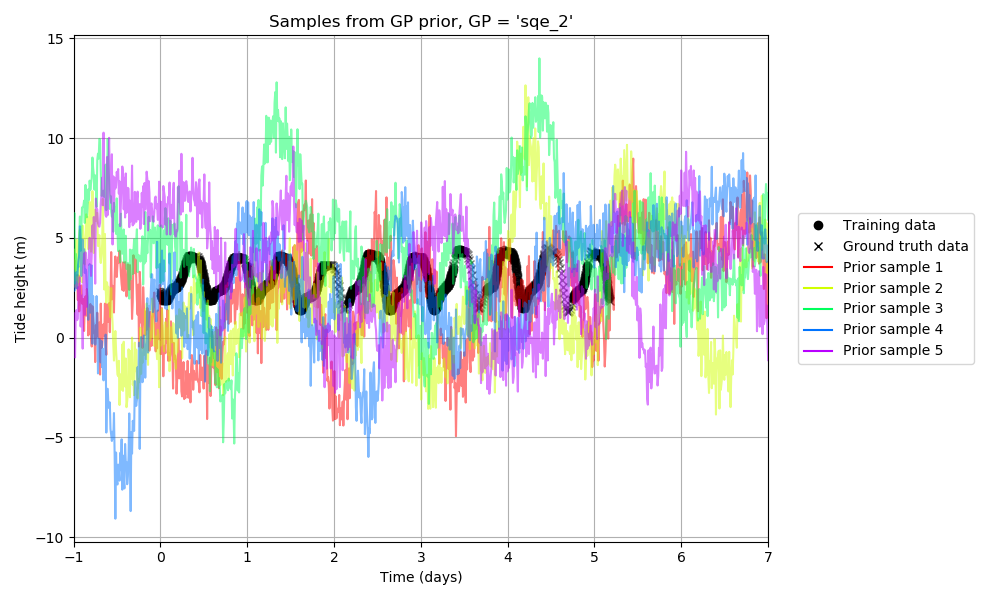
\includegraphics[width=0.45\textwidth]{Samples_from_GP_prior,_GP____sqe_2_.png}
    }
    \caption{Samples from the prior distribution of Gaussian Processes with square exponential kernels}
    \label{fig:prior_samples}
\end{figure}

% Figure: SQE predictive distribution

\begin{figure}[pht]
    \centering
    \subfloat[
        \centering Predictive distribution of sqe\_1
        \label{fig:pred_distribution_sqe_1}
    ]{
        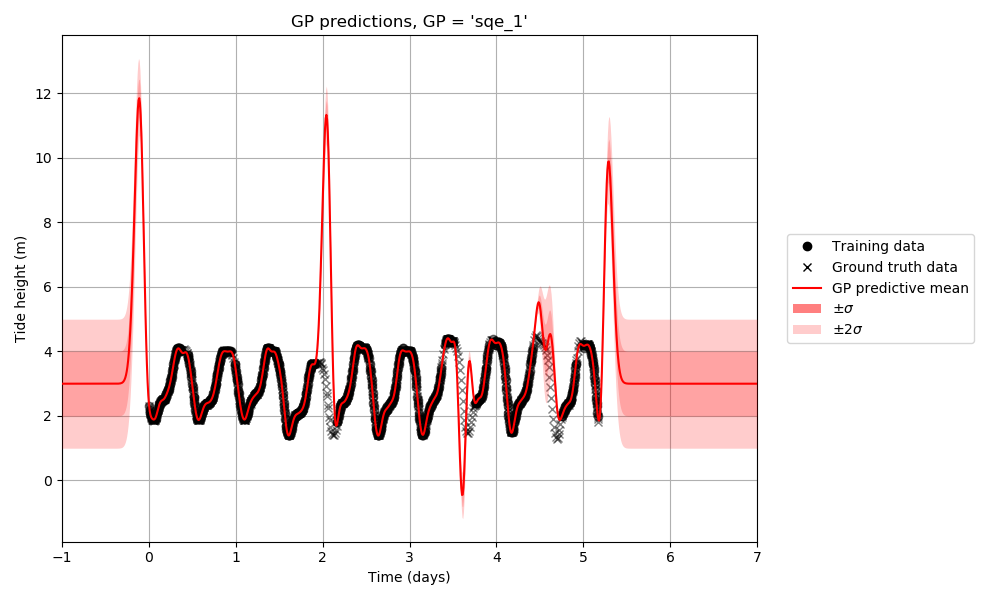
\includegraphics[width=0.45\textwidth]{GP_predictions,_GP____sqe_1_.png}
    }
    \subfloat[
        \centering Predictive distribution of sqe\_2
        \label{fig:pred_distribution_sqe_2}
    ]{
        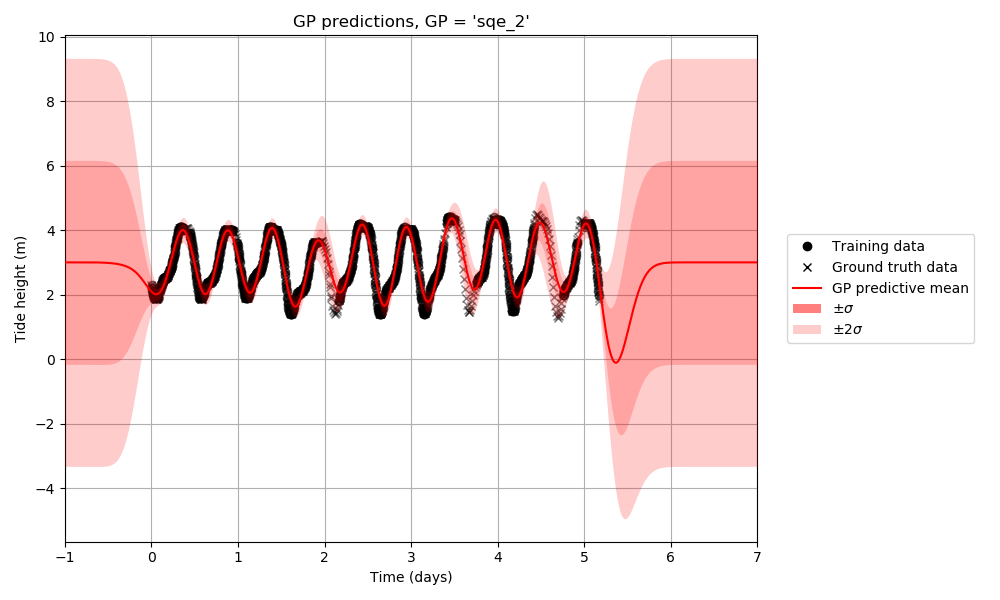
\includegraphics[width=0.45\textwidth]{GP_predictions,_GP____sqe_2_.png}
    }
    \caption{Predictive distributions of Gaussian Processes with square exponential kernels}
    \label{fig:pred_distribution}
\end{figure}

% Figure: SQE predictive samples

\begin{figure}[pht]
    \centering
    \subfloat[
        \centering Predictive distribution of sqe\_1
        \label{fig:pred_samples_sqe_1}
    ]{
        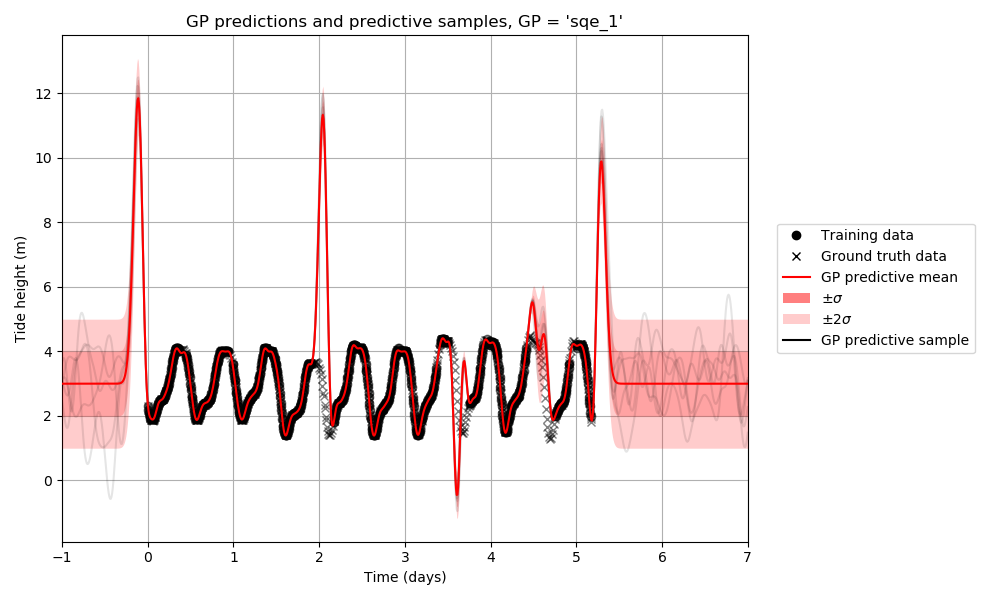
\includegraphics[width=0.45\textwidth]{GP_predictions_and_predictive_samples,_GP____sqe_1_.png}
    }
    \subfloat[
        \centering Predictive distribution of sqe\_2
        \label{fig:pred_samples_sqe_2}
    ]{
        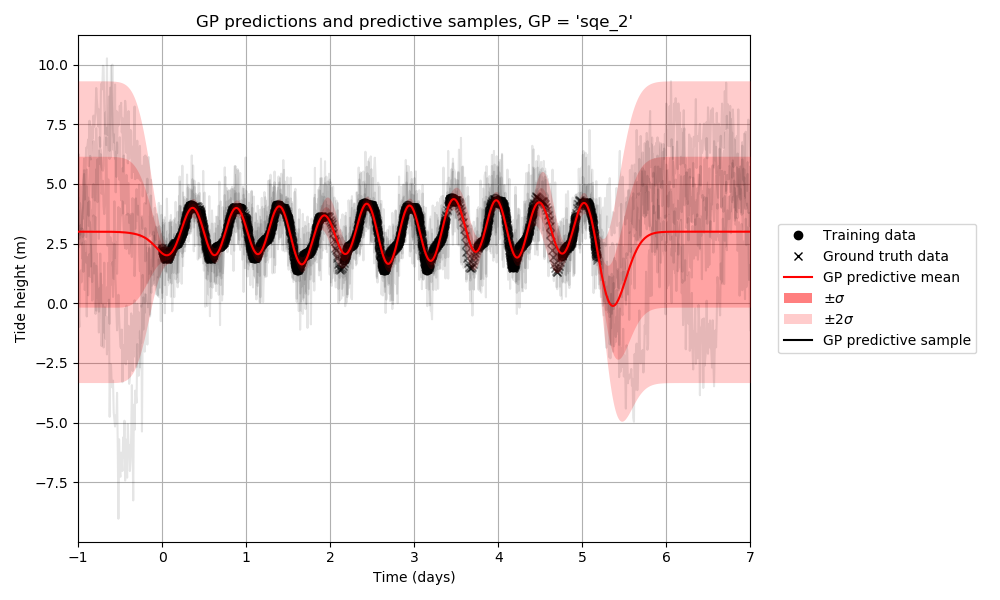
\includegraphics[width=0.45\textwidth]{GP_predictions_and_predictive_samples,_GP____sqe_2_.png}
    }
    \caption{Predictive distributions of Gaussian Processes with square exponential kernels}
    \label{fig:pred_samples}
\end{figure}

% Section: GP tables

\section{Description of Gaussian Processes used}\label{appendix:gp_table}

% Table: SQE Gaussian processes

\begin{table}[ht]
\centering
\begin{tabular}{|c|c|c|c|c|c|}
\hline
GP name  & $c$   & $\lambda$ & $k$    & $\sigma$ & LML       \\
\hline
sqe\_1   & 3     & 0.1       & 1      & 0.001    & -649119.3 \\
sqe\_2   & 3     & 0.3       & 10     & 1        & -1817.3   \\
sqe\_opt & 2.990 & 0.08665   & 0.6522 & 0.02931  & 1574.4    \\
\hline
\end{tabular}
\caption{Description of Gaussian Processes with squared exponential kernel that were evaluated in this report, and their log marginal likelihoods (LML)}
\label{table:sqe_table}
\end{table}


\section{Motivation for maximising the log marginal likelihood}\label{appendix:why_lml}

% References and end of document

\bibliographystyle{plain}
\bibliography{references}

\end{document}
